\documentclass{article}

\usepackage{graphicx}
\usepackage{tikz}
\usepackage{tikzsymbols}
\usetikzlibrary{calc,patterns,shapes.geometric}
\pagestyle{empty}
\usepackage[margin=0pt]{geometry}
\geometry{papersize={14in,12in}}

\def\centerarc[#1](#2)(#3:#4:#5){\draw[#1] ($(#2)+({#5*cos(#3)},{#5*sin(#3)})$) arc (#3:#4:#5);}

\begin{document}
	\begin{figure}
		\centering
		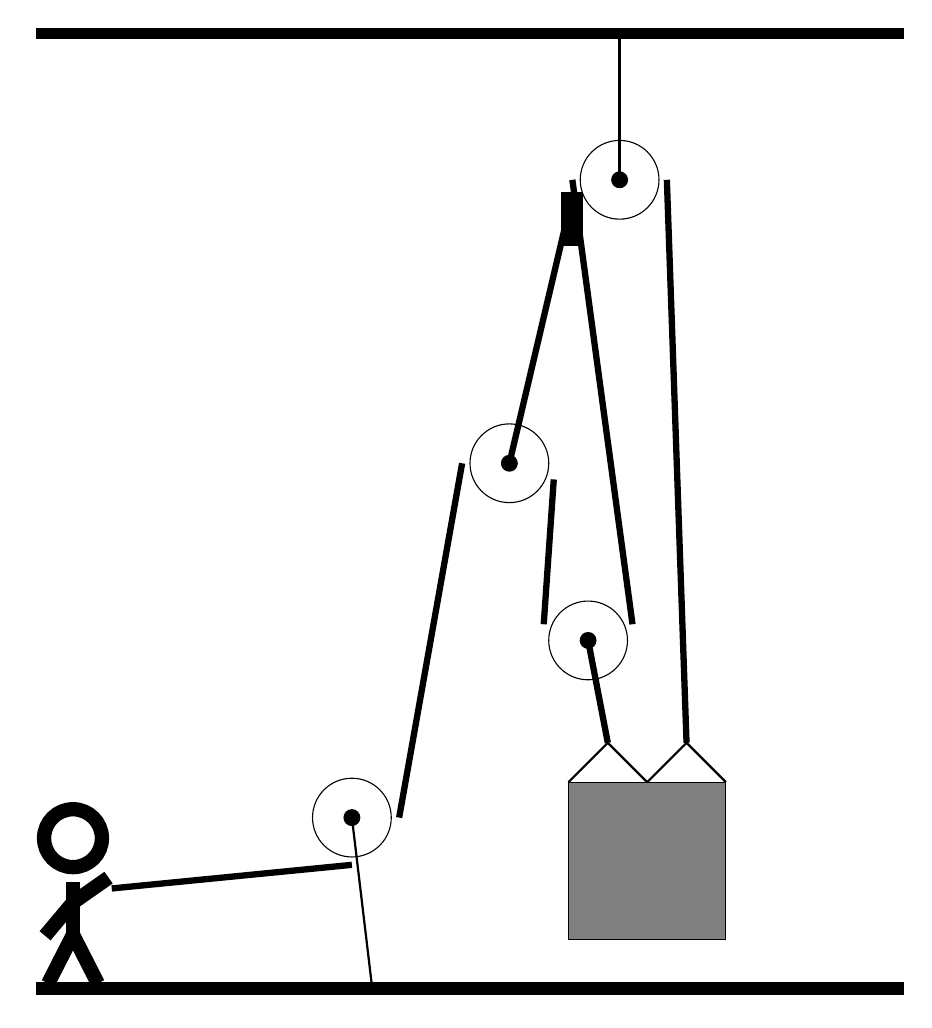
\begin{tikzpicture}
			%%%%% START %%%%%
			\draw[fill=black] (-6, 9) rectangle (5, 9.125);
			
			\draw (0, 3.6) circle (0.5);
			\draw[fill=black] (0, 3.6) circle (0.1);
			
			\draw (1, 1.35) circle (0.5);
			\draw[fill=black] (1, 1.35) circle (0.1);
			
			\draw (1.4, 7.2) circle (0.5);
			\draw[fill=black] (1.4, 7.2) circle (0.1);
			\draw[very thick] (1.4, 7.2) -- (1.4, 9);
			
			\draw (-2, -0.9) circle (0.5);
			\draw[fill=black] (-2, -0.9) circle (0.1);
			\draw[thick] (-2, -0.9) -- (-1.75, -3);
			
			
			\draw[thick]  (0.75, -0.45) -- (1.25, 0.05) -- (1.75, -0.45) -- (2.25, 0.05) -- (2.75, -0.45);
			\draw[fill=black!50] (0.75, -0.45) rectangle (2.75, -2.45);
			\draw[line width=0.8mm] (-5.05, -1.8) -- (-2, -1.5);
			\centerarc[line width=0.8mm](-2, -0.9)(270:360:0.6);
			\draw[line width=0.8mm] (-1.4, -0.9) -- (-0.6, 3.6);
			\draw[line width=0.8mm] (0, 3.6) -- (0.8, 7.0);
			\draw[line width=0.8mm, fill=black](0.7, 6.4) rectangle (0.9, 7.0);
			\centerarc[line width=0.8mm](0, 3.6)(-20:180:0.6);
			\draw[line width=0.8mm] (0.5638, 3.3948) -- (0.4362, 1.5552);
			\centerarc[line width=0.8mm](1, 1.35)(160:380:0.6);
			\draw[line width=0.8mm] (1.5638, 1.5552) -- (0.8, 7.2);
			\draw[line width=0.8mm](1, 1.35) -- (1.25, 0.05);
			\centerarc[line width=0.8mm](1.4, 7.2)(0:180:0.6);
			\draw[line width=0.8mm] (2.0, 7.2) -- (2.25, 0.05);
			
			\node at (-5.5, -1.9) {\Strichmaxerl[10][50][35]};
			
			\draw[fill=black] (-6, -3) rectangle (5, -3.15);
			%%%%% END %%%%%
		\end{tikzpicture}
	\end{figure}	
\end{document}